%priprava posamezne ure
%tukaj zaporedoma napisemo{st. zaporedne ure}{datum}{naslov}{poglavje}{oblika dela}{pripomocki}
\begin{priprava}{}{}{Kombinatorika}{Osnovni izrek kombinatorike}{frontalna}{tabla}

Motivacija:
\begin{itemize}
    \item (OSNOVNI PRIMER za \textbf{pravilo produkta}) V omari imamo 3 hlače, 4 puloverje in 2 pokrivali. Na koliko načinov se lahko oblečemo?
    
    Rešujemo kar z risanjem \textbf{kombinatoričnega drevesa} = grafičen prikaz vseh možnosti. Ugotovimo, da je odgovor $ 3 \cdot 4 \cdot 2 = 24 $.

    \begin{figure}[h]
        \centering
        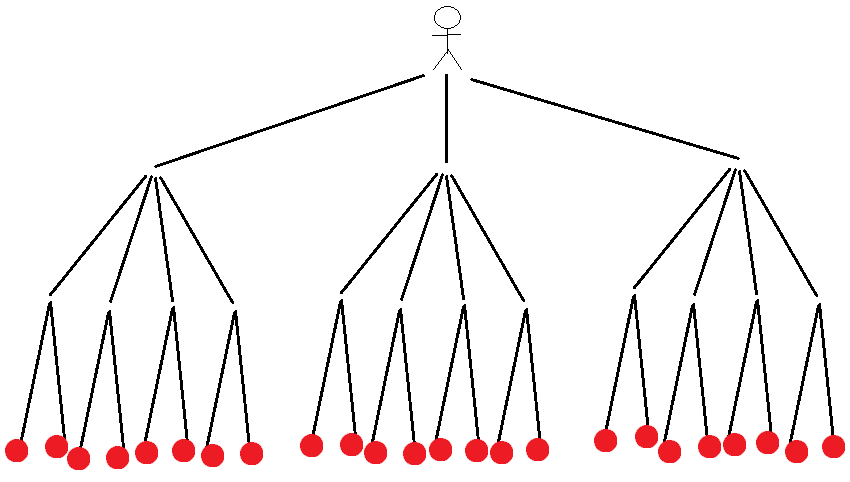
\includegraphics[width=0.7\textwidth]{slike/produkt.png}
    \end{figure}

    \item (OSNOVNI PRIMER za \textbf{pravilo vsote}) V omari imamo 3 dolge in 4 kratke hlače. Na koliko načino se lahko oblečemo?
    
    Na $ 3 + 4 = 7 $ načinov.
\end{itemize}

Kombinatorika je enostavno kar preštevanje.

\didopomba{Naslednji pravili sprotoma povezuj s primeroma od prej}

\textbf{Osnovni izrek kombinatorike ali pravilo produkta:} Imamo proces odločanja, sestavljen iz $ k $ zaporednih faz. V prvi fazi lahko sprejmemo $ n_1 $ odločitev, v drugi $ n_2 $ \ldots, v $ k $-ti pa $ n_k $ odločitev. Odločanje v vsaki fazi je neodvisno od prejšnjih odločitev. Število vseh sestavljenih odločitev je produkt vseh odločitev v posameznih fazah:
$$ N = n_1 \cdot n_2 \cdot n_3 \cdot \ldots \cdot n_k $$

\textbf{Pravilo vsote:} Če izbiramo med $ n_1 $ možnostmi iz prve množice \underline{ali} $ n_2 $ možnostmi iz druge množice \underline{ali} \ldots $ n_k $ možnostmi iz $ k $-te množice in so izbori iz vsake množice nezdružljivi z izbori iz drugih množic, potem je vseh izborov:
$$ M = n_1 + n_ 2 + \ldots + n_k $$

\newpage

Še primer kombinacije teh dve pravil:
\begin{itemize}
    \item Na koliko načinov si lahko oblečem 3 dolge ali 4 kratke hlače in 2 majici. \didopomba{pomoč s slikco}
    
    $ 3 \cdot 2 + 4 \cdot 2 = (3 + 4) \cdot 2 = 14 $
    
    \begin{figure}[h]
        \centering
        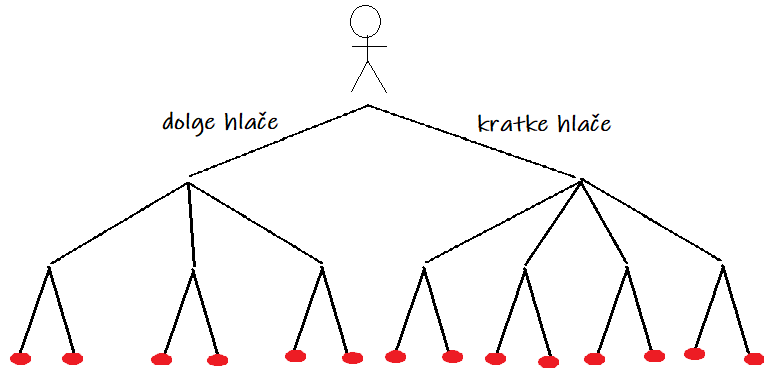
\includegraphics[width=0.7\textwidth]{slike/produktinvsota.png}
    \end{figure}

\end{itemize}

\vaje{
Vaje:
\begin{itemize}
    \item registrske tablice (gl. učbenik)
    \item razne vaje za vsako pravilo posebej in za kombinacijo obeh pravil
\end{itemize}
}
    
\didopomba{Za naprej -- ta poimenovanja, ``variacije'', ``kombinacije'' itd. pač oznake zanje pač omeni, ker je treba, ma point mora biti na tem, da znajo s kmečko pametjo rešit primer in ne razmišljat, a gre z variacije s ponavljanjem in kakšna je že formula ipd.}

\end{priprava}